% Chapter 4 - Design

\glsresetall % reset the glossary to expand acronyms again
\chapter[Design]{Application Development}\label{ch:Design}
\index{Design}

The Design is, as the name suggests, about the prototype or system you designed in order to achieve investigation or development goals of your research objective. The Design chapter is something that is typically found in engineering theses, hence our inclusion of that chapter. The scope and complexity of this chapter (or associated design chapters) depends on the level of the project: obviously a BSc final year project is going to be smaller scale and less complicated than a MSc project.

Commonly, systems that are built nowadays, and this relates especially to computer engineering or mechatronics types projects (but is relevant to many electrical engineering project too), involve multiple aspects.  Typically: (a) the System Level; (b) the Hardware Level and (c) the Software Level.  In addition, there may be considerations for the environment and/or `test rigs' (i.e., the infrastructure that may need to be set up around the system under test in order to perform the testing, and the test rig may in itself be a complicated system that needs thorough explanation.)

\section{System Design}
\label{sec:Design/SystemDesign}

As mentioned, the system you are designing may have multiple parts, both of the prototype and its surrounding test rig (you could call this `System Level Design' if you prefer, or something more accurate for your particular project).  The system level section of the design aims to explain what these big pieces or subsystems are that you are going to develop.  Often, for embedded systems particularly, the design is divided into a front-end and a back-end.

The front-end provides the point of interaction with other systems and/or the user.  A graphic user interface (GUI) may be part of the front-end (depending on the design) \ldots\ or the front-end might be signal conditioning and sampling electronics that then feeds into a front-end processor (e.g., FPGA) and further on into the system (e.g., towards back-end processing stages and storage). The user interface and GUI might be more in the back-end in some designs, e.g., a website services which the user or other programs connect to.

\emph{Note:} It is usually imperative to have a clear and easy-to-follow diagram (e.g., Fig.~\ref{fig:system_design}) to illustrate the system level and to refer to in your explanations for this section.

\begin{figure}[ht]
\centering
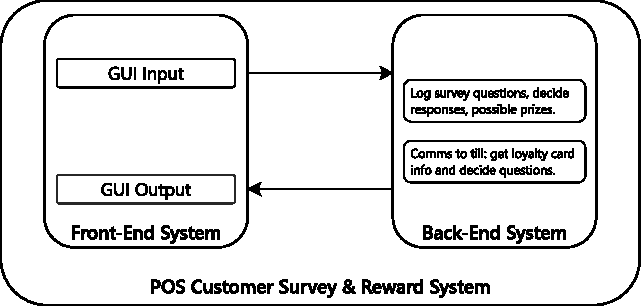
\includegraphics{3_Chapters/4_Chapter_Design/Figures/system_design.pdf}
\caption{Example system level design illustration}
\label{fig:system_design}
\end{figure}

The sections that follow the System Level depends on what your system involves. We have provided an example here of a system that has some Hardware Level aspects, some Software Level aspects and considerations for Integration (in this case setting up a test rig).

\section{Hardware Design}
\label{sec:Design/HardwareDesign}

The Hardware Design sections include significant details on your hardware design, PCB considerations, hardware interfacing and connections and power considerations, among other aspects that are specific to the hardware concerns of your prototype or system being built.  By `significant details' it is suggested that you do not need to go into excessive minutae of the design -- if you are building a significant piece of hardware largely from scratch, then you probably need a good amount of details to explain your choices etc.  You can also use an appendix in which to park information that may be providing extraneous detail that you think is nevertheless needed but is causing the write-up to become too bulky.

\emph{Note:} Even if your project is entirely software, you may still want to have a Hardware section to explain what platform and related components you were using; such information can help others to recreate your experiments, which are a desirable property of a good thesis.  If you are doing software performance tests you would need to provide characteristics of the platform, thus another reason for having a hardware section (but if the hardware section is just there for platform specs, then you can keep the section pretty short, likely not needing more than a page).

It's generally a good idea to include a block diagram and or schematics at this point.  Do not simply have a text-heavy discussion of what parts were used with a detailed schematic and photo of the hardware device that was built (doing so would offload the explanations and logical progression from design to PCB to the examiner to figure out, which is certainly not an advisable approach even if it saves much space).

A representative block diagram, which provides a clear explanation of a specific piece of a design, is presented in Fig.~\ref{fig:POS_Network}.  This figure was drawn in \href{http://www.inkscape.org/}{InkScape}~\cite{InkScape}. When you want to import an InkScape figure (SVG format) into \LaTeX{}, simply save it to PDF (use the drawing extents as the media box area) and include the figure.  This template includes a \texttt{`make figures'} target meant for this purpose.

\begin{figure}[ht]
\centering
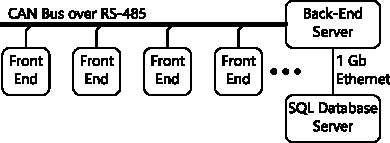
\includegraphics[scale=1.2]{3_Chapters/4_Chapter_Design/Figures/POS_Network.pdf}
\caption{Example hardware level design illustration}
\label{fig:POS_Network}
\end{figure}

\section{Software Design}

The software design section should go from the high-level design aspects, using for example block diagrams or UML class diagrams to explain the main parts of the system, and then going into details of specific operations or algorithms using some or a combination of, for example, pseudocode, UML state charts, UML activity diagrams, flow charts, or other appropriate figures to help the explanations.

You might decide to have some actual code (usually not more than code snippets, i.e., not whole programs) in the Software section, or you might decide to put such details into an implementation section (since the code is something that carries the design into an instantiated implementation).

Things you may have in the Software section include the following:

\begin{itemize}
  \item Software designs drawings (e.g., block diagrams, UML diagrams, etc.)
  \item Algorithms (maybe in pseudocode, or actual code such as MATLAB)
  \item Code snippets (where relevant, used to illustrate how you went from algorithm, or an element of the software design, to executable implemented code)
  \item Implementation and development methods (for example specific software tools that had to be installed, scripts to run, parameters to use; but remember that some of this particular item may be better placed in the methodology -- particularly if it relates to choices that were made earlier on or even before development started.)
\end{itemize}

\section{Implementation}

For a project that is largely hardware based, the implementation section is sometimes rather short, providing photos of the system and explaining some tips and methods on how it was put together (e.g., solutions that were learned for how to solder on parts effectively, or through the implementation experience realising parts that need to be handled with special care etc.) For a project that involves hardware and software, this section could include both tips on getting the hardware together, as well as details about implementing the software.

\section{Integration or Test Rig}

Some research projects require the development of surrounding infrastructure or a suitably conditioned or prepared environment in order to carry out the testing. This may involve developing some sort of test rig into which the prototype is placed or coupled so that testing can be performed on it.  As a simple example, consider a vibration measuring device. If you want to test it in the lab, which has concrete floors but you want to test it for a range of flooring types, it may be necessary to build one or more test rigs that will provide the needed characteristics in order to test the product in a sufficiently authentic situation.

The integration section may alternatively, or in addition to the above point, explain how different subsystems of the system constructed are connected up.  For example, this section might be used to explain the different ways to connect up a system that combines some software on a PC, a complicated DSP platform, and perhaps separate front-end conditioning circuitry, in order to complete experiments to test the achievement of different sub-objectives of the project.
